%!TEX root = ../thesis.tex

\section{Shrinking chords}
In this section we will explain the operation of \emph{shrinking chords}.


Suppose that during sweeping we find a chord  in our candidate walk. Then we are in the situation of Figure \ref{fig:chord:situation}.

\begin{figure}[h]
  \centering
  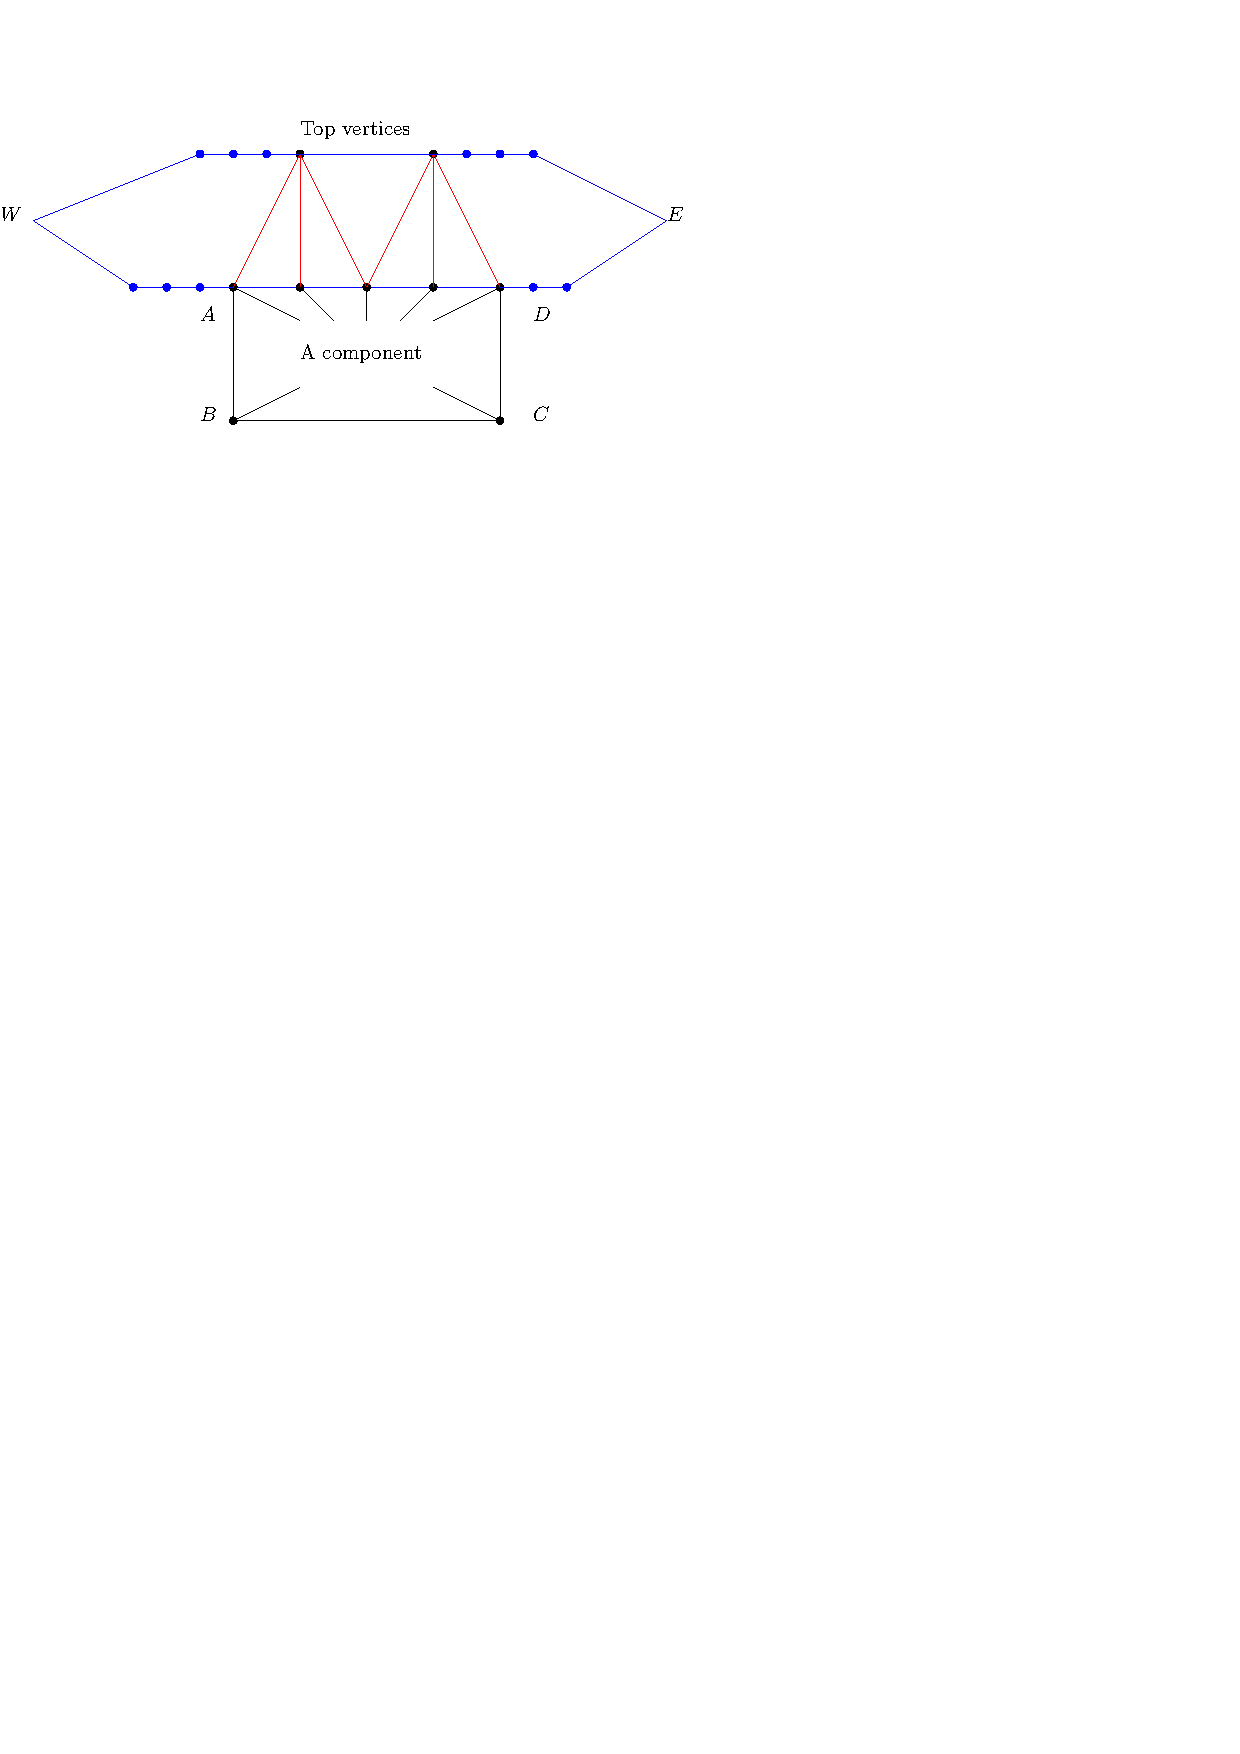
\includegraphics[scale=1]{chordShrink/img/situation}
  \caption{}
  \label{fig:chord:situation}
\end{figure}

We make a case distinction on the number of edges going from A and B to the component. We make a distionction between both having only 1 edge. One have 1 edge and 1 having more edges and both having more edges.


\subsection{Both one edge}

If both have only one edge both these edge will go to the same vertex $v$ and this vertex must also be adjacent to $A$ and $D$. This makes $AvD$ a 2-chord. Since the sweepcycle doesn't admit any seperating 2-chords we know the rest must be exactly as drawn. We escape the chord by departing at $B$ and taking the path $BvD$.
See also Figure \ref{fig:chord:oneonefan}.

\begin{figure}[h]
  \centering
  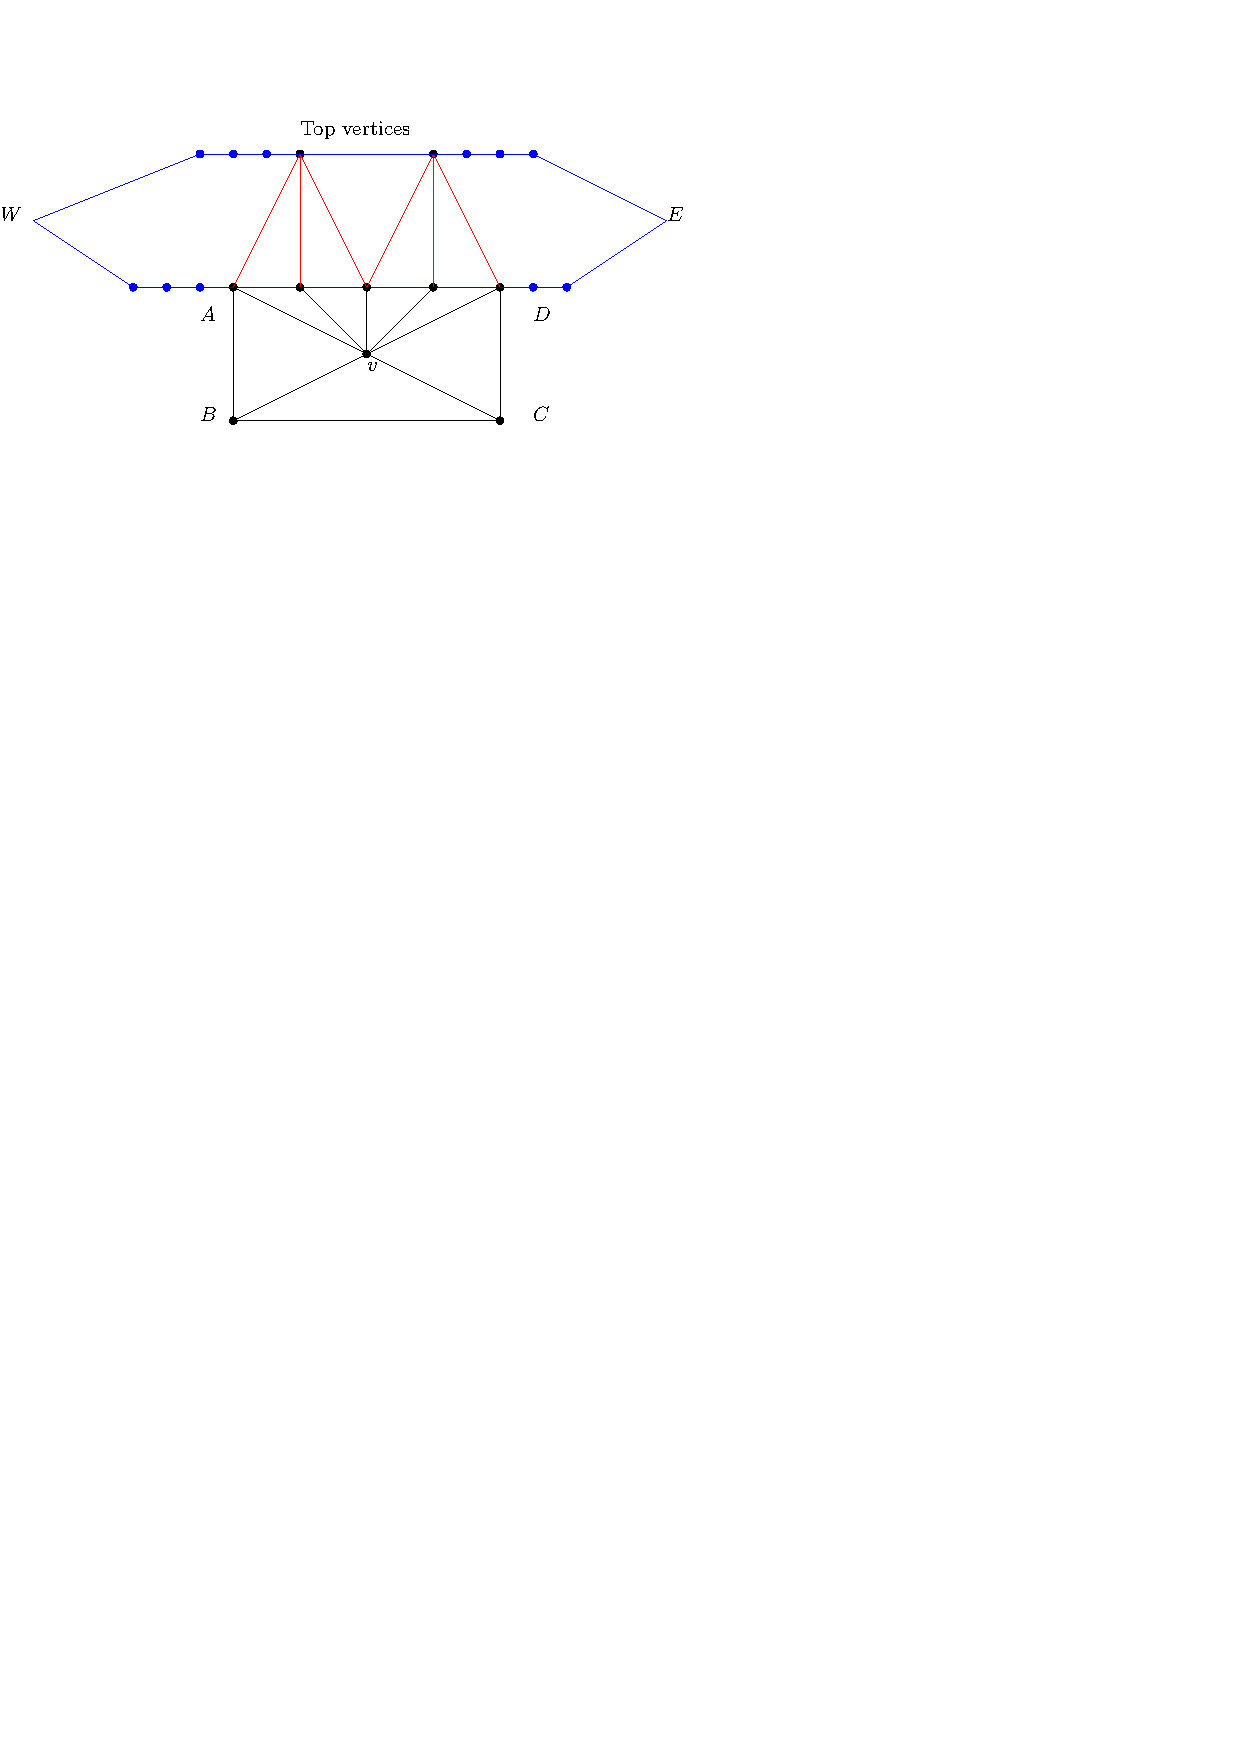
\includegraphics[scale=1]{chordShrink/img/oneonefan}
  \caption{}
  \label{fig:chord:oneonefan}
\end{figure}


\subsection{Both more then one edge}

If both have more then one edge we shrink the entire interior of the bold \fxwarning{TODO} cycle to a single point and we arrive at the situation in Figure \ref{fig:chord:shrink}. The numbers in the right part are the ranges the edge counts must have at that point.

\begin{figure}[h]
  \centering
  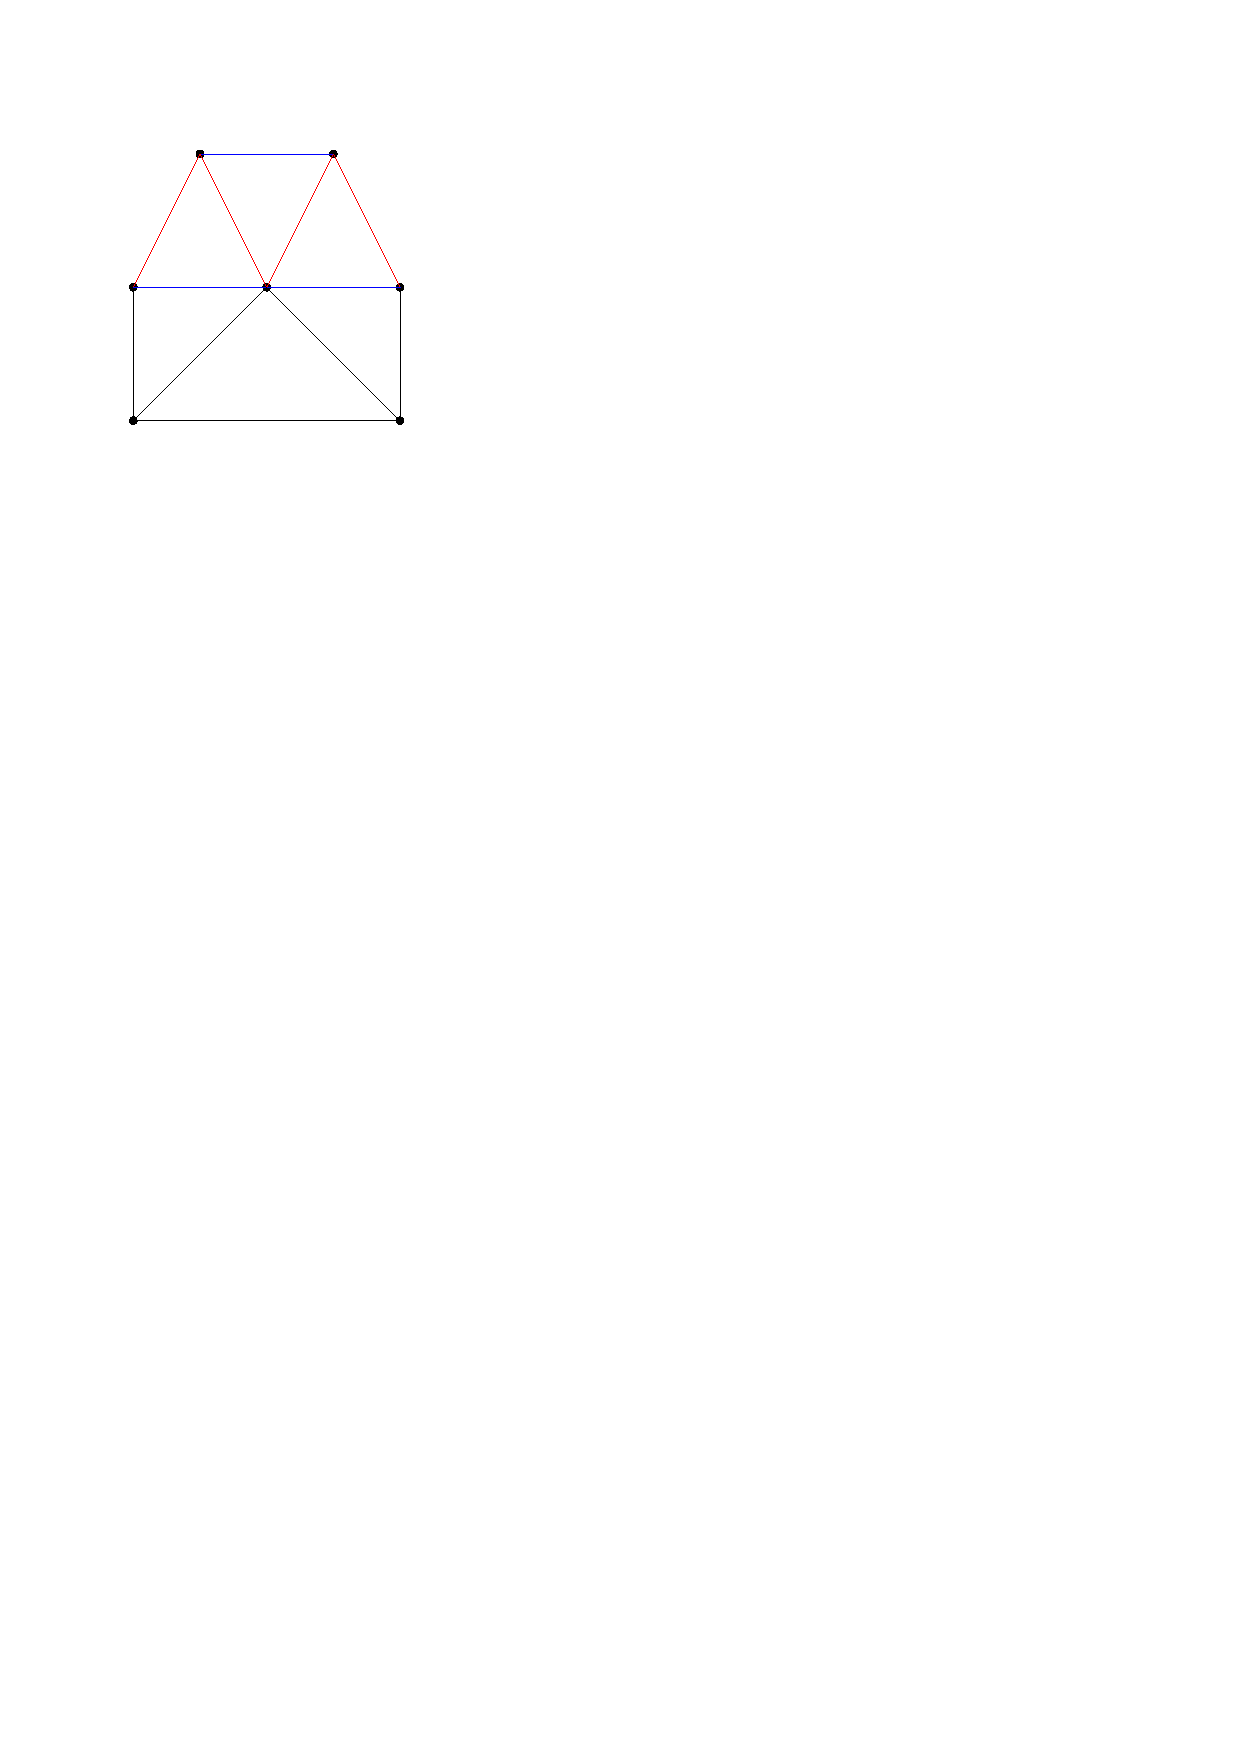
\includegraphics[scale=1]{chordShrink/img/shrink}
  \caption{Applying the shrink}
  \label{fig:chord:shrink}
\end{figure}

%We always do this for a \emph{maximal} chord. That is a chord whose \emph{range} is not contained in the range of any other chord.

We then have the following Lemma's.

\begin{lemma}
  \label{lm:}fan
  The shrink does not create a seperating triangle.
\end{lemma}

\begin{proof}
  A separating triangle would be created if two nonadjecent vertices would be connected by an edge.

  A connection between two topvertices would be an chord in an earlier valid path. This is forbidden. A connection between a top vertex and A, B, C or D Would also intersect a sweepline. Wich is impossible.

  An connection $AC$ or $BD$ would give a separating $2-$chord on the sweepline. Which is something we avoid.

  Hence the shrink can't create a separating triangle.
\end{proof}



\begin{lemma}
  \label{lm:}
  The shrink does not create any $4$-cycles that are wholly on or below the sweepcycle.
\end{lemma}

\begin{proof}
  Such an cycle $\C$ would be created by an 2 edge connection between $A$ and $C$, $B$ and $D$ or $A$ and $D$. The last one would imply a seperating 2-chord on the sweepcyle, so this can't be.

  The other two would imply a larger chord containing the chord $BC$. However we took the largest chord.
\end{proof}

Any 4-cycle partially above the 4-cycle doens't infuence the solvability of this graph badly. Since the part of the graph is above the sweepcycle is functionally the same as a large North vertex. \fxwarning{TODO Make this rigorous?}

More rigorously we could show that these things don't affect or possibility to find new valid paths.


\subsection{One has one edge and the other one more}
This is the most complicated situation. If there is one vertex with only one edge going into an interior component, then this edge goes to a vertex which we will denote by $v$.

\subsubsection{B has only one edge}
We see that $AvCD$ is also a 3-chord. If it is a separating chord we recurse on this chord. Otherwise we color it like in the figure. Depending on the result of that recursion we shrink it or we recurse again.

In any case we color as in the Figure \ref{}. This is exceptional as we're adding paths while not in that point in the algorithm. And even more exceptionall because they are splits not adjacent to $S$ but due to the oustide chord their location and size is very controlled. 
\fxwarning{TODO we also check neighbour count of A}

\subsubsection{C has only one edge}
We see that $ABvD$ is also a 3-chord. If it is a separating chord we recurse on this chord.
